\documentclass[a4paper, 12pt, slovene]{article}
\usepackage[slovene]{babel}
\usepackage[utf8]{inputenc}
\usepackage{lmodern}
\usepackage[T1]{fontenc}
\usepackage{graphicx}
\usepackage{caption}
\captionsetup{font=footnotesize}
\usepackage{fullpage}
\usepackage{enumitem}
\usepackage{array}
\usepackage{wrapfig}
\usepackage{multirow}
\usepackage{tabularx}
\usepackage{amsmath}
\usepackage{amssymb}
\usepackage{subcaption}
\newcommand*\diff{\mathop{}\!\mathrm{d}}
\newcommand*\Diff[1]{\mathop{}\!\mathrm{d^#1}}
\newcommand*\difft{\mathop{}\!\ddot{ }}
\usepackage{float}
\usepackage{mathrsfs}



\newcommand{\Ai}{\mathrm{Ai}}
\newcommand{\Bi}{\mathrm{Bi}}

\renewcommand{\Re}{\mathop{\rm Re}\nolimits}
\renewcommand{\Im}{\mathop{\rm Im}\nolimits}
\newcommand{\Tr}{\mathop{\rm Tr}\nolimits}
\newcommand{\diag}{\mathop{\rm diag}\nolimits}
\newcommand{\dd}{\,\mathrm{d}}
\newcommand{\ddd}{\mathrm{d}}
\newcommand{\ii}{\mathrm{i}}
\newcommand{\lag}{\mathcal{L}\!}
\newcommand{\ham}{\mathcal{H}\!}
\newcommand{\four}[1]{\mathcal{F}\!\left(#1\right)}
\newcommand{\bigO}[1]{\mathcal{O}\!\left(#1\right)}
\newcommand{\sh}{\mathop{\rm sinh}\nolimits}
\newcommand{\ch}{\mathop{\rm cosh}\nolimits}
\renewcommand{\th}{\mathop{\rm tanh}\nolimits}
\newcommand{\erf}{\mathop{\rm erf}\nolimits}
\newcommand{\erfc}{\mathop{\rm erfc}\nolimits}
\newcommand{\sinc}{\mathop{\rm sinc}\nolimits}
\newcommand{\rect}{\mathop{\rm rect}\nolimits}
\newcommand{\ee}[1]{\cdot 10^{#1}}
\newcommand{\inv}[1]{\left(#1\right)^{-1}}
\newcommand{\invf}[1]{\frac{1}{#1}}
\newcommand{\sqr}[1]{\left(#1\right)^2}
\newcommand{\half}{\frac{1}{2}}
\newcommand{\thalf}{\tfrac{1}{2}}
\newcommand{\pd}{\partial}
\newcommand{\Dd}[3][{}]{\frac{\ddd^{#1} #2}{\ddd #3^{#1}}}
\newcommand{\Pd}[3][{}]{\frac{\pd^{#1} #2}{\pd #3^{#1}}}
\newcommand{\avg}[1]{\left\langle#1\right\rangle}
\newcommand{\norm}[1]{\left\Vert #1 \right\Vert}
\newcommand{\braket}[2]{\left\langle #1 \vert#2 \right\rangle}
\newcommand{\obraket}[3]{\left\langle #1 \vert #2 \vert #3 \right \rangle}
\newcommand{\hex}[1]{\texttt{0x#1}}

\renewcommand{\iint}{\mathop{\int\mkern-13mu\int}}
\renewcommand{\iiint}{\mathop{\int\mkern-13mu\int\mkern-13mu\int}}
\newcommand{\oiint}{\mathop{{\int\mkern-15mu\int}\mkern-21mu\raisebox{0.3ex}{$\bigcirc$}}}

\newcommand{\wunderbrace}[2]{\vphantom{#1}\smash{\underbrace{#1}_{#2}}}

\renewcommand{\vec}[1]{\overset{\smash{\hbox{\raise -0.42ex\hbox{$\scriptscriptstyle\rightharpoonup$}}}}{#1}}
\newcommand{\bec}[1]{\mathbf{#1}}



\begin{document}

\begin{titlepage}
\title{\textsc{FFT in Avtokorelacije} \\[1ex] \large Peta naloga pri predmetu Matematično-fizikalni praktikum}
\author{Gašper Lotrič, 28191019}
\date{4. november 2021}

\maketitle
\end{titlepage}

\tableofcontents
\pagebreak


\section{Uvod}
Diskretno Fourierovo transformacijo smo definirali kot
\begin{equation*}
H_k = \sum_{n=0}^{N-1}
h_n \exp(2 \pi \ii k n / N),
\qquad k=-\tfrac{N}{2},\dots ,\tfrac{N}{2},
\end{equation*}
oziroma
\begin{equation*}
H_k = \sum_{n=0}^{N-1} W_N^{nk} h_n,
\qquad W_N = \exp(2 \pi \ii / N).
\end{equation*}
Ta postopek ima očitno časovno zahtevnost $N^2$. Račun pa je
mogoče izvesti tudi z bistveno manj operacijami. Osnovni premislek
je razcep
\begin{equation*}
H_k = H_{k}^\mathrm{sod} + W_N^k H_{k}^\mathrm{lih} \>,  
\end{equation*}
kjer smo transformiranko $H$ izrazili s transformacijama njenih
sodih in lihih členov, pri čemer je vsota vsake od transformacij zdaj dolžine N/2.
 Gornjo relacijo lahko uporabljamo rekurzivno:
če je $N$ enak potenci števila 2, lahko rekurzijo razdrobimo
do nizov, ki imajo samo še en člen. Zanj je transformacija
identiteta. Za obrat pri eni vrednosti frekvence (pri danem $m$)
je potrebno na vsakem koraku rekurzije le eno množenje s potenco
$W$, korakov pa je $\log_2 N$.  Skupna časovna zahtevnost je torej
le še $N\log_2 N$.

Da ne iščemo pripadnikov niza po vsej tabeli, si podatke
preuredimo. Lahko je pokazati, da je v prvotni tabeli treba med
seboj zamenjati podatke, katerih vrstna števila v binarnem zapisu
so obrnjena: v novem redu jemljemo člene kar po vrsti. Tudi
potenc $W$ ne izražamo vedno znova s sinusi in kosinusi,
pač pa jih računamo z rekurzijo.  Tak ali podoben postopek
je osnova vseh algoritmov hitre Fourierove transformacije (FFT).

Z neko transformacijo iz družine FFT bomo izračunali korelacijsko
funkcijo dveh signalov. Korelacija periodičnih funk\-cij $g(t)$ in $h(t)$
s periodo $T$ je definirana kot:
\begin{equation*}
\phi_{gh}(\tau)=\frac{1}{T}\int\limits_0^{T} g(t+\tau)\,h(t)\dd t \>,  
\end{equation*}
oziroma diskretno
\begin{equation*}
  \phi_{gh}(n)= \frac{1}{N}\sum_{k=0}^{N-1} g_{k+n}\, h_k \>.
\end{equation*}
Računamo torej skalarni produkt funkcij, ki sta časovno premaknjeni
za $\tau$ oziroma $n$. Če je za določeno vrednost premika ta
funkcija višja kot v okolici, potem to pomeni, da sta si funkciji
podobni, le da ju je treba premakniti, da se to vidi.

V primeru, da sta funkciji (signala), ki ju primerjamo, enaki,
računamo njuno {\sl avtokorelacijsko funkcijo\/}: ta je mera
za to, ali signal ostaja s pretekanjem časa sam sebi podoben.
Če je signal slabo koreliran (sam s sabo), korelacija $\phi_{hh}(n)$
relaksira h kvadratu povprečnega signala $\langle h\rangle^2$, kjer je
\begin{equation*}
\langle h\rangle = \frac{1}{N} \sum_{k=0}^{N-1} h_k \>.  
\end{equation*}
Iz lokalnih maksimov v avtokorelacijski funkciji sklepamo
na periodičnosti, bodisi popolne ali približne.
Pri periodičnih signalih je tudi avtokorelacijska funkcija
striktno periodična, za stohastične procese pa je značilna
eksponentna avtokorelacijska funkcija.
še bolj nas zanima, kako {\sl hitro\/} se korelacija izgublja:
računamo rajši reskalirano obliko avtokorelacije
\begin{equation*}
\widetilde{\phi}_{hh}(n) = 
{ \phi_{hh}(n) - \langle h\rangle^2 \over \phi_{hh}(0) - \langle h\rangle^2 } \>,  
\end{equation*}
kjer je imenovalec nekakšno merilo za  varianco signala,
\begin{equation*}
\sigma^2 = \phi_{hh}(0) - \langle h\rangle^2 
= \frac{1}{N} \sum_{k=0}^{N-1} \left( h_k - \langle h\rangle \right)^2 \>.  
\end{equation*}
Pri zgornjih enačbah moramo še ``peš'' poskrbeti za periodično
zaključenost signala pri $n=N$, torej da je perioda enaka velikosti
vzorca.  Če tega ne moremo narediti, je bolj pravilna definicija
avtokorelacije
\begin{equation*}
\phi_{hh}(n)= \frac{1}{N-n}\sum_{k=0}^{N-n-1} h_{k+n}\, h_k \>.  
\end{equation*}
Praktičen račun po zgornji formuli lahko postane za velike
vzorce prezamuden.  Avtokorelacijo rajši računamo s FFT (DFT) $\mathcal{F}$,
saj je korelacija obratna Fourierova transformacija ${\cal F}^{-1}$
produkta Fourierovih transformacij ${\cal F}$, torej z $G={\cal F}g$ in $H={\cal F}h$ dobimo
\begin{equation*}
\phi_{gh}(n) = \frac{1}{N-n}\mathcal{F}^{-1} \left[ G \cdot (H)^\ast \right]
\end{equation*}
oziroma
\begin{equation*}
  \phi_{hh}(n) = \frac{1}{N-n}{\cal F}^{-1} \left[ \, | H |^2 \, \right] \>.
\end{equation*}
Za račun s FTT signale dolžine $N$ najprej prepišemo v dvakrat
daljše, periodično zaključene podatkovne nize, $\widetilde{h}_n = h_n$,
$\widetilde{h}_{n+N} = 0$ za $n = 0, \ldots, N-1$
in $\widetilde{h}_{n+2N} = \widetilde{h}_{n}$.
Tedaj se avtokorelacija zapiše v obliki
\begin{equation*}
\phi_{hh}(n)={1\over N-n}\sum_{k=0}^{2N-1}\widetilde{h}_{k+n}\,\widetilde{h}_k \>,  
\end{equation*}
kar lahko izračunamo s FFT.

\section{Naloga}

Na spletni strani MF praktikuma najdeš posnetke
oglašanja velike uharice, naše največje sove.  Posneti sta
dve sovi z minimalnim ozadjem ({\tt bubomono} in {\tt bubo2mono})
in nekaj mešanih signalov, ki zakrivajo njuno oglašanje
({\tt mix}, {\tt mix1}, {\tt mix2} in {\tt mix22}).
V signalih {\tt mix2} in {\tt mix22} je oglašanje sove
komaj še zaznavno.  Izračunaj avtokorelacijsko funkcijo 
vseh signalov in poskusi ugotoviti, za katero sovo gre
pri teh najbolj zašumljenih signalih!

Priporočamo uporabo rutine {\tt four1\/} iz Numerical Recipes
ali knjižnice {\tt fftw3}, ki je še dosti hitrejša. V okolju Python
so te rutine vključene v 'fft' paket. 
(Pri tako velikih vzorcih je skorajda nujno uporabiti FFT
namesto počasne navadne DFT.)

\bigskip

\subsection{Dodatna naloga}
Izračunaj še avtokorelacijsko funkcijo za kak signal, ki ga posnameš sam ali za kak proces, za katerega sam poiščeš ustrezne podatke.



\section{Algoritem FFT}
Časovno zahtevnost in odvisnost napake od števila vzorčenj bom preveril na funkciji, zliženi iz raznih sinusnih in cosinusnih valovanj. \par\vspace{5mm}

Nekaj prednosti hitre fourierove transformacije glede na navaden diskretni algoritem sem pokazač že pri prejšnji nalogi. Tam sem predvsem govoril o hitrosti algoritmov in kako FFT z $\mathcal{O}(n\log n)$ hitro pokaže svjo moč napran počasnejšim algoritmom s časovno odvisnostjo $\mathcal{O}(n^2)$. Preveril bom še kako je s časovno zahtevnostjo računanja (avto)korelacijske funkcije. Za števila vzorčenj vrednosti $2^n$ ima ta funkcija časovno odvisnost $\mathcal{O}(n\log n)$. \par\vspace{5mm}

\begin{figure}[H]
\centering
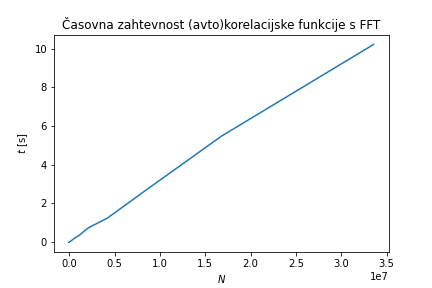
\includegraphics[width=0.7\textwidth]{grafi/kor-cas.png}
\caption{Časovna zahtevnost avtokorelacijske funkcije.}
\label{f:time}
\end{figure}

Ker pri računanju korelacij signalov uporabimo Fourierovo transformacijo in nato še inverzno Fourierovo transformacijo, je pomembno, da je transformacija natančna. To bom preveril s primerjavo originalnega signala z inverzno transformiranko njegove transformiranke. Na sliki \ref{f:napaka} napaka implementacije DFT iz četrte naloge, kljub absolutno majhnim vrednostim, narašča linearno s številom vzorčenj, napaka FFT pa ostaja majhna. 

\begin{figure}[H]
\centering
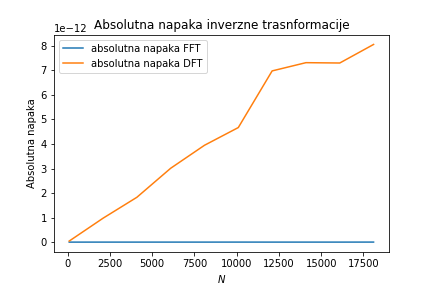
\includegraphics[width=0.7\textwidth]{grafi/napake.png}
\caption{Napaka inverzne Fourierove transformacije.}
\label{f:napaka}
\end{figure}



\section{Oglašanje sov}
V tem razdelku naloge bom analiziral posnetke oglašanja dveh različnih sov. V začetnih dveh posnetkih sta jasna zvoka dveh različnih sov uharic, potem pa imam še štiri posnetke, kjer je njuno uhanje zamaskirano za raznimi šumi (tabela \ref{t:zvoki}). Moj cilj je določiti, katera sove se oglaša v katerem posnetku. Najprej si bom pogledal frekvenčne spektre vseh posnetkov. \par\vspace{5mm}

\begin{table}[H]
\centering
\begin{tabular}{|c|c|}
\hline
posnetek & zvoki \\
\hline
\texttt{bubomono.wav}	&	Sova (Alja)	\\
\texttt{bubo2mono.wav}	&	Sova (Branko)	\\
\texttt{mix.wav}	&	Sova, črički	\\
\texttt{mix1.wav}	&	Sova, črički, potok	\\
\texttt{mix2.wav}	&	Sova, črički, veter	\\
\texttt{mix22.wav}	&	Sova, deroča reka	\\
\hline
\end{tabular}
\caption{Kaj slišimo na posnetkih. Na čistih posnetkih sov je jasno, da sta različni, kasneje pa ne vem katera se oglasi.}
\label{t:zvoki}
\end{table}

\begin{figure}[H]
\centering
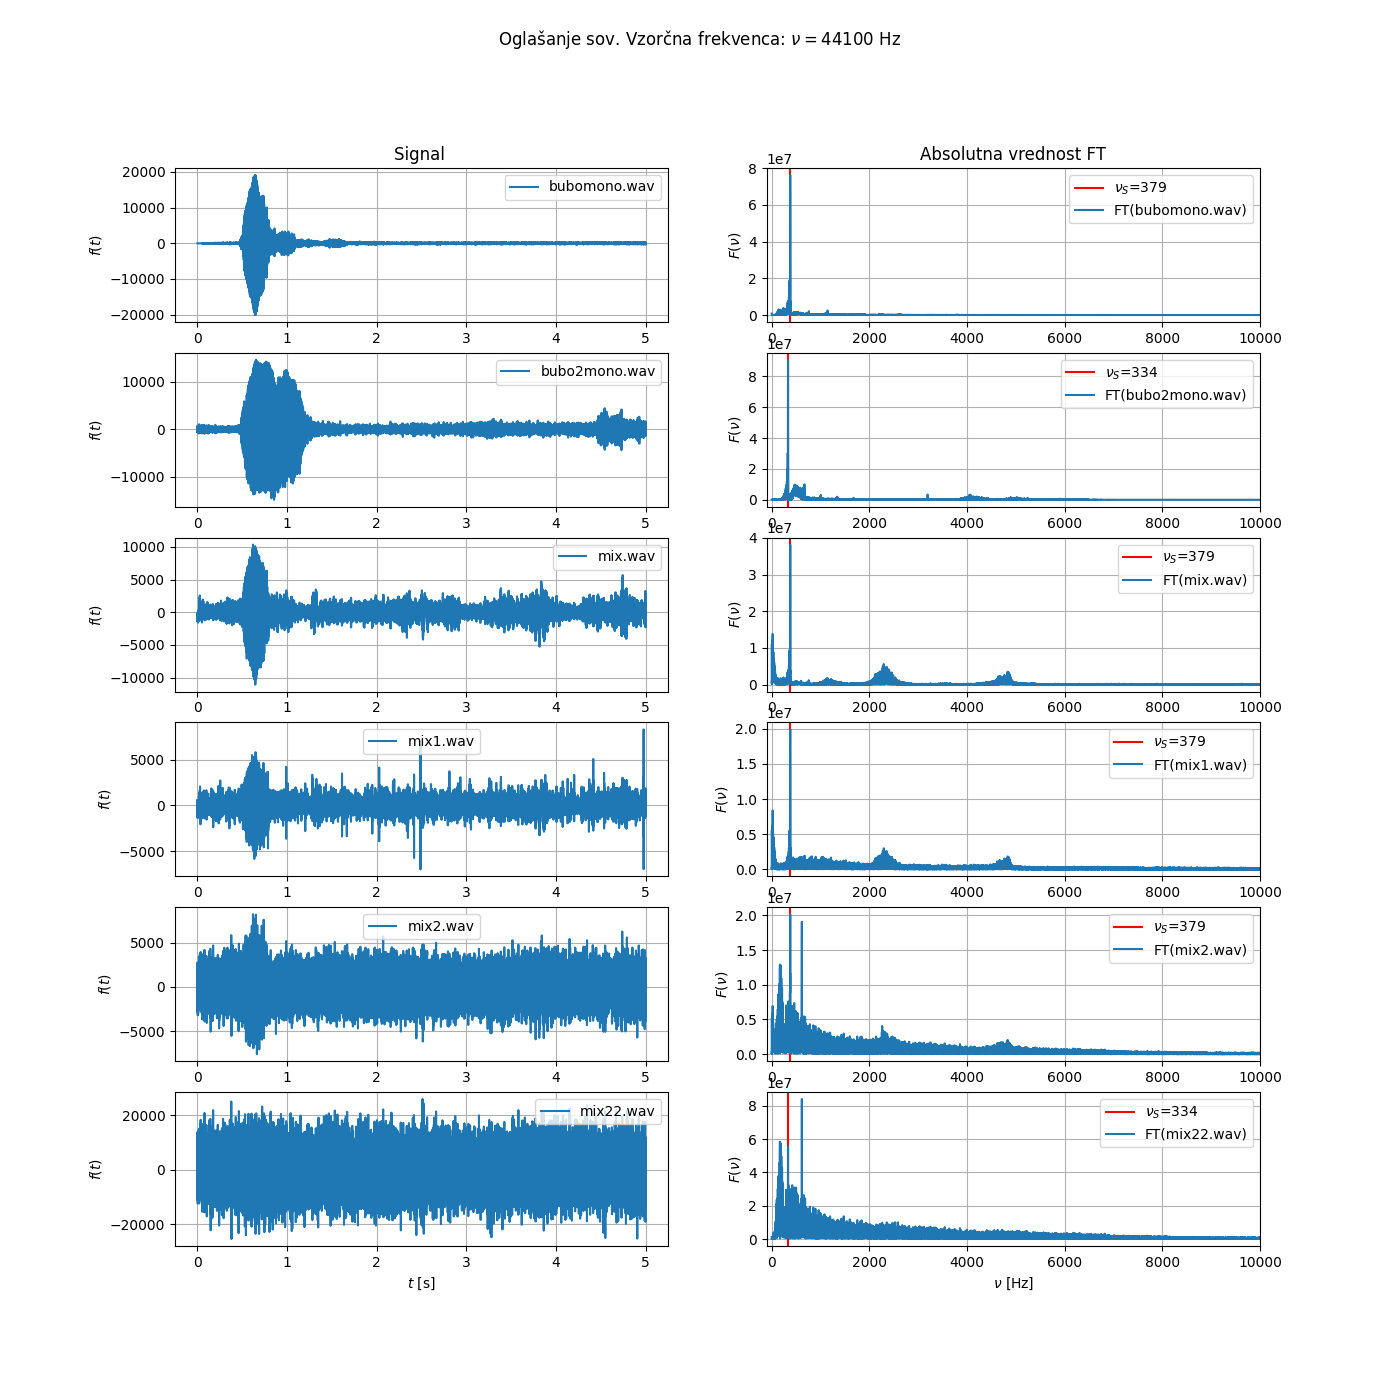
\includegraphics[width=0.90\textwidth]{grafi/sove.png}
\caption{Signal in fourierova transformacija oglašanja sov z različnimi ozadji.}
\label{f:sove}
\end{figure}

Na fekvenčnih spektrih na sliki \ref{f:sove} vidimo, da se obe sovi oglašata z relativno nizkimi frekvencami 334 Hz in 379 Hz, visokih frekvenc pa je na čistih posnetkih zelo malo. Pozorno oko opazi tudi, da se prva sova oglaša z mlce višjo frekvenco. Z dodajanjem šuma dodajamo vse več frekvenc v celem spektru. Zanimivo je, da se v posnetkih, kjer so prisotni črički vidi ''kupček'' ojačitev še pri dveh frekvencah (ker je drugi ravno pri dvakratnikau prvega, gre lahko za višje harmonike). Za razliko pa je spkter reke vliko bolj zvezen. \par\vspace{5mm}

Ker se sovi oglašata pri različnih frekvencah, sem ju enostavno ločil tako, da sem pogledal najmočnejšo frekvenco v vskem zvočnem posnetku (pri zadnjem tretji največji vrh). V posnetkih \texttt{mix, mix1, mix2} in \texttt{bubomono} se oglaša ena sova (Alja), v posnetkih \texttt{mix22} in \texttt{bubo2mono} pa druga (Branko).


\subsection{Avtokorelacija}
Z avtokorelacijsko funkcijo računamo, če signal s časom ostaja sam sebi podoben. V tem primeru vemo, da to ne bo res, saj se sovi oglasita le za kratek čas. Zato bosta avtokorelacijski funkciji hitro padali s časom. \par\vspace{5mm}

\begin{figure}[H]
\centering
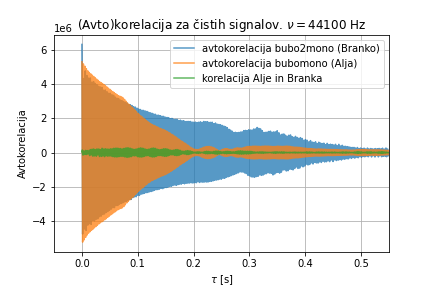
\includegraphics[width=0.7\textwidth]{grafi/avtokorelacija-sove-lim.png}
\caption{Avtokorelacijska funkcija za obe sovi in korelacija med njima.}
\label{f:autokor-sove}
\end{figure}

Na sliki \ref{f:autokor-sove} sta prikazani avtokorelacijski funkciji za vsako od velikih uharic ter korelacijska funkcija med njima. Kot pričakovano, avtokorelacija hitro pade v obeh primerih. Pri Branku se po zaključku skovikanja pojavijo še neki zvoki, zato je avtokorelacijska funkcija nekoliko sedlasta preden spet začne strmo padati. Korelacijska funkcija pa je skozi celoten časovni interval skoraj ničelna. Zdaj sem dobil orodje, da se lahko lotim prepoznavanja sov na drugačen način.


\subsection{Korelacije}
Ker so vsi mešani posnetki narejeni iz samostojnih posnetkov sov in se začnejo naenkrat, lahko privzamem, da je v vseh primerih $\tau = 0$ (sove se oglasijo v obeh posnetkih naenkrat). Primerjal bom signala Alje in Branka z ostalimi zašumljenimi posnetki. \par\vspace{5mm}

\begin{figure}[H]
\centering
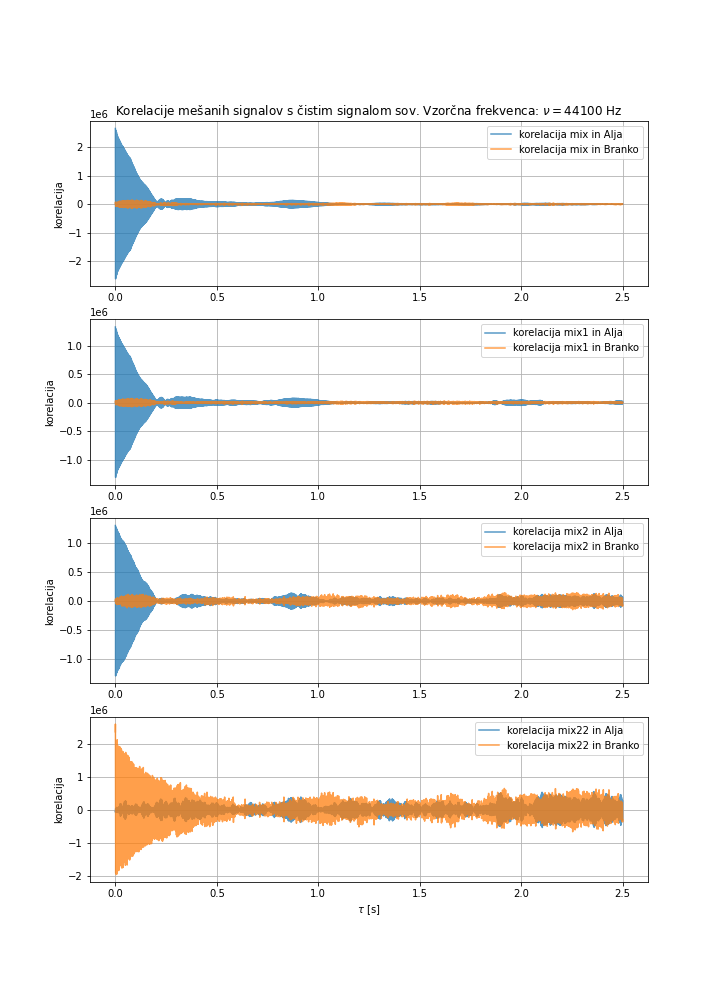
\includegraphics[width=0.71\textwidth]{grafi/korelacije.png}
\caption{Korelacije med mešanimi signali in originalnimi skovikanji.}
\label{f:korelacije-sove}
\end{figure}

Na sliki \ref{f:korelacije-sove} so prikazane korelacije zašumljenih posnetkov z eno in drugo sovo. Zdaj je veliko bolj enostavno razbrati, katera sova se kje oglaša. Ne glede na zašumljenost ozadja so bili signali iste sove vedno korelirani in signala različih sov nekorelirana. Pravzaprav sem sestavil amatersko verzijo aplikacije Shazam.



\section{Sončeve pege}
Za dodatno nalogo sem izbral analizosignala sončevih peg (sunspots). Sončeve pege so pojavi na površju Sonca, ki jih zaznamo kot temnejša območja. Te pege so območja z nižjo temperaturo, kjer magnetni tok otežuje konvekcijo. Normalno se pojavijo v parih in vztrajajo od nekaj dni do par mesecev, potem pa izginejo. Njihovo skupno število pa ima periodo približno 11 let. \par\vspace{5mm}

\begin{figure}[H]
\centering
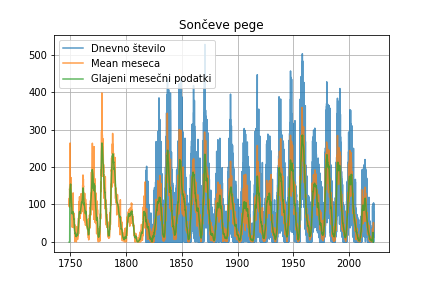
\includegraphics[width=0.7\textwidth]{grafi/sunspots.png}
\caption{Signali sončevih peg.}
\label{f:sunspots}
\end{figure}

Podatke o sončevih pegah sem dobil na spletni strani \cite{soncne-pege}. Imajo zbrane podatke za vsak dan, potem pa še obdelane za obdobja mesecev in let. Nihanje števila sončevih peg sem predstavil na sliki \ref{f:sunspots}. Signali izgledajo periodični, ampak je težko razbrati, kaj se dogaja. Da je perioda res 11 let, bom preveril s pomočjo avtokorelacijske funkcije. 

\begin{figure}[H]
\centering
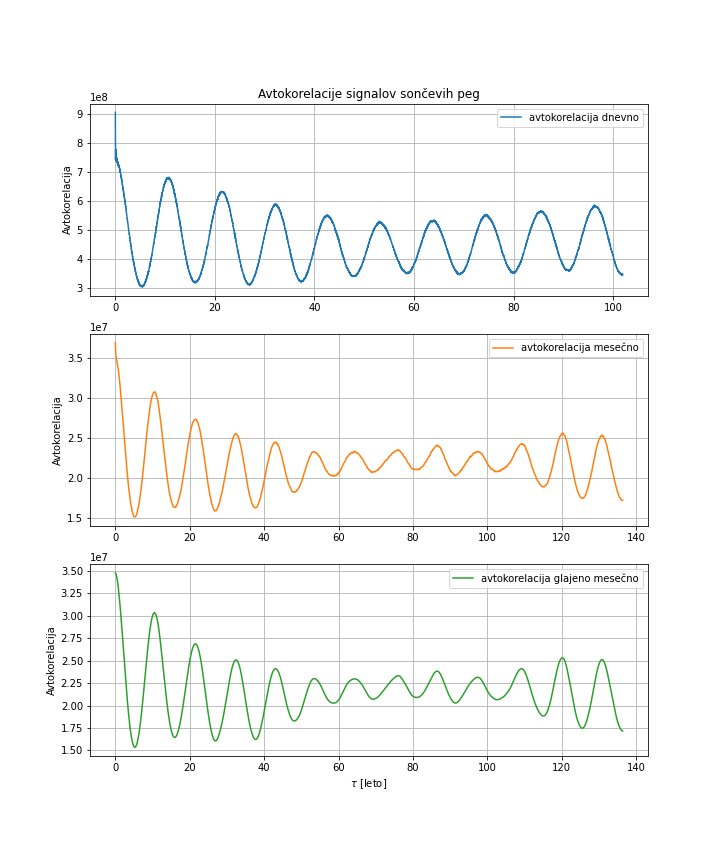
\includegraphics[width=0.71\textwidth]{grafi/avtokorelacija-sunspots.png}
\caption{Avtokorelacije signalov sončevih peg merjenih na različnih intervalih.}
\label{f:sunspots-autocorr}
\end{figure}

Pri avtokorelacijah signalov je perioda sončevega cikla lepo opazna in lahko vidimo, da je re enaka 11 let.
 

\section{Zaključek}
V tej nalogi sem se dobro seznanil z uporabo FFT. Ta lagoritem je od normalne diskretne FT bistveno hitrejši in od moje metode tudi natančnajši. Razliko v hitrostih lahko opazimo že ''na oko''. \par\vspace{5mm}

Z uporabo FFT in IFFT sem izračunal korelacijsko funkcijo in jo uporabil za avtokorelacijo signalov in korelacijo med signali.  Ker ta funkcija ''meri'' podobnost signalov, je avtokorelacijska funkcija periodičnih signalov prav tako periodična. Tako sem na primeru časovne odvisnosti sončevih peg iz podatkov lahko razbral periodo približno 11 let., ko aktivnost doseže maksimum. \par\vspace{5mm}

Korelacija med dvema signaloma se je izkazala kot močno orodje za razpoznavanje signalov iz zašumljenega ozadja. To sem spoznal na testnem primeru dveh sov. na podoben način bi lahko naredil prepoznavanje glasbe, motivov na slikah in podobno. Za dodatno nalogo sem veliko razmišljal o prepoznavanju črk na slikah (računalniški vid) ampak na koncu sklenil, da je ta 60 let star problem preveč za današnji večer.


\begin{thebibliography}{9}

\bibitem{soncne-pege} 
Sunspot Index and Long-term Solar Observations
\\\texttt{https://wwwbis.sidc.be/silso/datafiles}

\end{thebibliography}



\end{document}
